\documentclass[a4paper,11pt]{article}

\usepackage[T1]{polski}
\usepackage[utf8]{inputenc} 
\usepackage{graphicx}
\usepackage{float}
\usepackage{verbatim}
\hoffset=-3.0cm                 % Mniejszy lewy margines
\textwidth=18cm                 % szerzej
\evensidemargin=0pt

\voffset=-3cm                   % Mniejszy gorny margines
\textheight=27cm                % szerzej wzdluz

\usepackage{listings}
% Listingi
\lstdefinestyle{customc}{
	belowcaptionskip=1\baselineskip,
	breaklines=true,
	frame=L,
	xleftmargin=0pt,
	language=HTML,
	showstringspaces=false,
	basicstyle=\footnotesize\ttfamily,
	identifierstyle=\color{black}
}

\setlength{\parindent}{0pt}             % No paragraph indentation
\setlength{\parskip}{\medskipamount}    % Space between paragraphs
\raggedbottom   


\title{POLITECHNIKA WARSZAWSKA \\ WYDZIAŁ ELEKTRYCZNY \\}
\author{Michał Sut}
\date{\today}

\begin{document}
	\thispagestyle{empty}
	\maketitle
	\date{}
	\section{Treść zadania}
		Napisać program rozwiązujący problem komiwojażera (minimalizacja drogi pomiędzy n miastami bez powtórzeń) przy pomocy algorytmu genetycznego. Zastosować reprodukcję przy użyciu nieproporcjonalnej ruletki, operator krzyżowania CX oraz mutację równomierną.\\~\\
		Program powinien umożliwiać użycie różnych wielkości populacji, liczby iteracji, prawdopodobieństwa mutacji.
		\\~\\
		Program powinien zapewnić wizualizację wyników w postaci wykresów średniego, maksymalnego i minimalnego przystosowania (długości funkcji) dla kolejnych populacji oraz 2 map (o wymiarach 10x10 punktów), na których będą wyświetlane miasta oraz drogi najdłuższa i najkrótsza.
		\\~\\
		Pokazać działanie programu na danych testowych składających się z 10 miast, opisanych za pomocą współrzędnych na mapie o wymiarach 10x10 punktów.
		\\~\\
		Dane testowe: miasta:\\
		A(4,4), B(1,1), C(8,9), D(2,10), E(4,10), F(6,9), G(5,6), H(1,8), I(8,7), J(9,4)
	\section{Instrukcja działania programu}
		\subsection{Uruchomienie}
			Program został napisany w języku Python, z wykorzystaniem bibliotek zawartych w dystrybucji Anaconda3. W związku z tym, należy uruchamiać program w tym środowisku. Można to zrobić poprzez zaimportowanie projektu do programu Visual Studio 2017, wybranie interpretera: Anaconda 4.2 i uruchomienie aplikacji. Plikiem startowym jest \texttt{ga.py}
		\subsection{Okno główne programu}
			\begin{figure}[H]
				\centering
				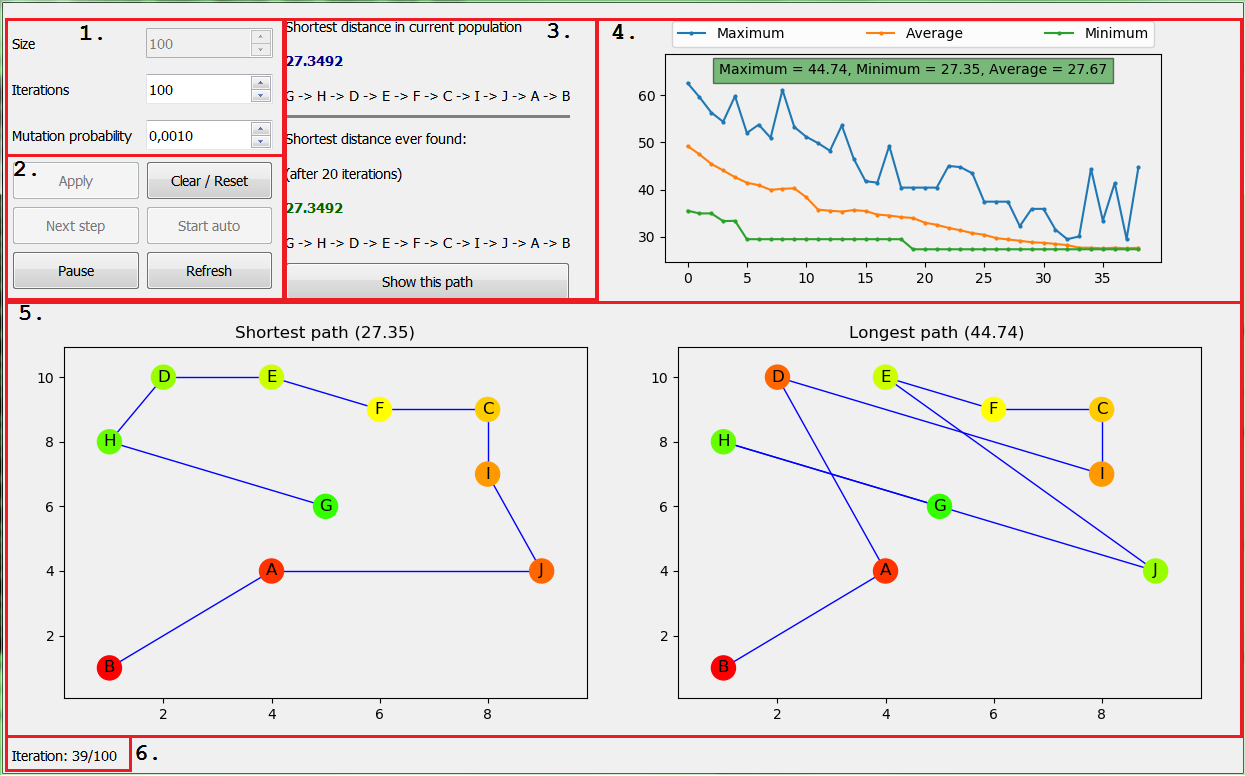
\includegraphics[scale=0.55]{main_window2.png}
			\end{figure}
		
		\subsection{Opis okna programu}
			\begin{enumerate}
				\item Parametry algorytmu
				\item Przyciski sterowania
				\item Informacje o najkrótszych znalezionych trasach
				\item Wykres wartości średnich, maksymalnych i minimalnych dla kolejnych generacji.
				\item Mapy z miastami i trasami: po lewej -- najkrótsza trasa, po prawej -- najdłuższa
				\item Informacja o numerze aktualnej iteracji
			\end{enumerate}
		
		\subsection{Zmiana ustawień programu}
			Ustawienia programu znajdują się w pliku \texttt{settings.py}. Zmianą podlegają następujące elementy:
			\begin{enumerate}
				\item \textbf{CITIES} - Nazwy miast
				\item \textbf{POSITIONS} - Współrzędne miast
				\item \textbf{COLORS} - Kolory jakimi zaznaczane są kolejne miasta
			\end{enumerate}
	
		\subsection{Użycie}
			\subsubsection{Podstawowe operacje}
				\begin{enumerate}
					\item Ustawić parametry populacji
					\item Zainicjować populację klikając przycisk \framebox{ \texttt{Apply}}
					\item W tym momencie dostępne są trzy możliwości:
					\begin{enumerate}
						\item \framebox{Next Step} - Wykonanie tylko jednej generacji
						\item \framebox{Start Auto} - Wykonywanie kolejnych n generacji, gdzie n jest wybraną liczbą iteracji
						\item \framebox{Clear/Reset} - Wyczyszczenie populacji i zresetowanie programu
					\end{enumerate}
					\item Rozpoczęty proces automatycznych generacji można wstrzymać przyciskiem \framebox{Pause}
					\item Aby zobaczyć najkrótszą kiedykolwiek znalezioną trasę należy brać przycisk \framebox{Show this path}
				\end{enumerate}
			
		\subsection{Warunek stopu}
		Program zatrzymuje się po określonej liczbie iteracji, którą użytkownik określa w panelu ustawień parametrów algorytmu. Liczbę iteracji można zwiększać w trakcie działania programu.
		
	\section{Opis eksperymentów}
	Eksperymenty przeprowadzone były dla miast o następujących współrzędnych:  $A(4,4), B(1,1), C(8,9), D(2,10), E(4,10), F(6,9), G(5,6), H(1,8), I(8,7), J(9,4)$.
%	 Dokładność znalezionego rozwiązania obliczona jest poprzez obliczenie stosunku znalezionej wartości maksymalnej do wartości obliczonej analitycznie. W tym przypadku, maksimum funkcji wynosi $47$ i jest osiągane dla argumentu $x = 20$
	
		\subsection{Różna liczebność populacji}
			W celu przeprowadzenia tych eksperymentów, kilkukrotnie uruchomiony zostanie algorytm z następującymi parametrami: prawdopodobieństwo mutacji -- 0,001, liczba iteracji -- 200.
			\subsubsection{Populacja: 10 osobników}
				Wyniki prezentują się następująco:\\~\\
				\begin{tabular}{|c|c|c|c|c|}
					\hline 
					Lp & Min & Max & Mean & Best \\
					\hline
					1 & 31,63  & 34,72 & 33,48 & 31,63\\\hline
					2 & 35,36 & 35,36  &35,36 & 35,36 \\\hline
					3 & 35,99 & 35,99  & 35,99 &34,15 \\\hline
					4 & 31,08 & 31,08  & 31,08& 31,08 \\\hline
					5 & 31,96 & 31,96  & 31,96 & 31,96\\\hline
					&avg. min:&avg. max:&avg. mean:&avg. best:\\\hline
					& 33,20 & 33,82& 33,57 &32,84\\\hline
				\end{tabular} 
				
%				TU KONTYNUOWAC! !! !  ! ! 

			\subsubsection{Populacja: 50 osobników}
				Wyniki prezentują się następująco:\\~\\
				\begin{tabular}{|c|c|c|c|c|}
					\hline 
					Lp & Min & Max & Mean & Best \\
					\hline
					1 & 31,63  & 34,72 & 33,48 & 31,63\\\hline
					2 & 35,36 & 35,36  &35,36 & 35,36 \\\hline
					3 & 35,99 & 35,99  & 35,99 &34,15 \\\hline
					4 & 31,08 & 31,08  & 31,08& 31,08 \\\hline
					5 & 31,96 & 31,96  & 31,96 & 31,96\\\hline
					&avg. min:&avg. max:&avg. mean:&avg. best:\\\hline
					& 33,20 & 33,82& 33,57 &32,84\\\hline
				\end{tabular} 
			\subsubsection{Populacja: 120 osobników}
				Wyniki prezentują się następująco:\\~\\
				\begin{tabular}{|c|c|c|c|c|}
					\hline 
					Lp & Min & Max & Mean & Best \\
					\hline
					1 & 31,63  & 34,72 & 33,48 & 31,63\\\hline
					2 & 35,36 & 35,36  &35,36 & 35,36 \\\hline
					3 & 35,99 & 35,99  & 35,99 &34,15 \\\hline
					4 & 31,08 & 31,08  & 31,08& 31,08 \\\hline
					5 & 31,96 & 31,96  & 31,96 & 31,96\\\hline
					&avg. min:&avg. max:&avg. mean:&avg. best:\\\hline
					& 33,20 & 33,82& 33,57 &32,84\\\hline
				\end{tabular} 
			\subsubsection{Populacja: 600 osobników}
				Wyniki prezentują się następująco:\\~\\
				\begin{tabular}{|c|c|c|c|c|}
					\hline 
					Lp & Min & Max & Mean & Best \\
					\hline
					1 & 31,63  & 34,72 & 33,48 & 31,63\\\hline
					2 & 35,36 & 35,36  &35,36 & 35,36 \\\hline
					3 & 35,99 & 35,99  & 35,99 &34,15 \\\hline
					4 & 31,08 & 31,08  & 31,08& 31,08 \\\hline
					5 & 31,96 & 31,96  & 31,96 & 31,96\\\hline
					&avg. min:&avg. max:&avg. mean:&avg. best:\\\hline
					& 33,20 & 33,82& 33,57 &32,84\\\hline
				\end{tabular} 
			\subsection{Różne prawdopodobieństwa krzyżowania}
				Eksperymenty przeprowadzone będą dla populacji 10 osobników, z prawdopodobieństwem mutacji równym 0.001
				\subsubsection{Krzyżowanie: prawdopodobieństwo = 1,00}
					Wyniki prezentują się następująco:\\~\\
					\begin{tabular}{|c|c|c|c|c|}
						\hline 
						Lp & Min & Max & Mean & Best \\
						\hline
						1 & 31,63  & 34,72 & 33,48 & 31,63\\\hline
						2 & 35,36 & 35,36  &35,36 & 35,36 \\\hline
						3 & 35,99 & 35,99  & 35,99 &34,15 \\\hline
						4 & 31,08 & 31,08  & 31,08& 31,08 \\\hline
						5 & 31,96 & 31,96  & 31,96 & 31,96\\\hline
						&avg. min:&avg. max:&avg. mean:&avg. best:\\\hline
						& 33,20 & 33,82& 33,57 &32,84\\\hline
					\end{tabular} 
				\subsubsection{Krzyżowanie: prawdopodobieństwo = 0,90}
					Wyniki prezentują się następująco:\\~\\
					\begin{tabular}{|c|c|c|c|c|}
						\hline 
						Lp & Min & Max & Mean & Best \\
						\hline
						1 & 31,63  & 34,72 & 33,48 & 31,63\\\hline
						2 & 35,36 & 35,36  &35,36 & 35,36 \\\hline
						3 & 35,99 & 35,99  & 35,99 &34,15 \\\hline
						4 & 31,08 & 31,08  & 31,08& 31,08 \\\hline
						5 & 31,96 & 31,96  & 31,96 & 31,96\\\hline
						&avg. min:&avg. max:&avg. mean:&avg. best:\\\hline
						& 33,20 & 33,82& 33,57 &32,84\\\hline
					\end{tabular} 
				\subsubsection{Krzyżowanie: prawdopodobieństwo = 0,50}
					Wyniki prezentują się następująco:\\~\\
					\begin{tabular}{|c|c|c|c|c|}
						\hline 
						Lp & Min & Max & Mean & Best \\
						\hline
						1 & 31,63  & 34,72 & 33,48 & 31,63\\\hline
						2 & 35,36 & 35,36  &35,36 & 35,36 \\\hline
						3 & 35,99 & 35,99  & 35,99 &34,15 \\\hline
						4 & 31,08 & 31,08  & 31,08& 31,08 \\\hline
						5 & 31,96 & 31,96  & 31,96 & 31,96\\\hline
						&avg. min:&avg. max:&avg. mean:&avg. best:\\\hline
						& 33,20 & 33,82& 33,57 &32,84\\\hline
					\end{tabular} 
				\subsubsection{Krzyżowanie: prawdopodobieństwo = 0,00}
					Wyniki prezentują się następująco:\\~\\
					\begin{tabular}{|c|c|c|c|c|}
						\hline 
						Lp & Min & Max & Mean & Best \\
						\hline
						1 & 31,63  & 34,72 & 33,48 & 31,63\\\hline
						2 & 35,36 & 35,36  &35,36 & 35,36 \\\hline
						3 & 35,99 & 35,99  & 35,99 &34,15 \\\hline
						4 & 31,08 & 31,08  & 31,08& 31,08 \\\hline
						5 & 31,96 & 31,96  & 31,96 & 31,96\\\hline
						&avg. min:&avg. max:&avg. mean:&avg. best:\\\hline
						& 33,20 & 33,82& 33,57 &32,84\\\hline
					\end{tabular} 
			\subsection{Różne prawdopodobieństwa mutacji}
				Eksperymenty przeprowadzone będą dla populacji 10 osobników, z prawdopodobieństwem krzyżowania równym 1,00
				\subsubsection{Mutacja: prawdopodobieństwo = 0,000}
					Wyniki prezentują się następująco:\\~\\
					\begin{tabular}{|c|c|c|c|c|}
						\hline 
						Lp & Min & Max & Mean & Best \\
						\hline
						1 & 31,63  & 34,72 & 33,48 & 31,63\\\hline
						2 & 35,36 & 35,36  &35,36 & 35,36 \\\hline
						3 & 35,99 & 35,99  & 35,99 &34,15 \\\hline
						4 & 31,08 & 31,08  & 31,08& 31,08 \\\hline
						5 & 31,96 & 31,96  & 31,96 & 31,96\\\hline
						&avg. min:&avg. max:&avg. mean:&avg. best:\\\hline
						& 33,20 & 33,82& 33,57 &32,84\\\hline
					\end{tabular} 
				\subsubsection{Mutacja: prawdopodobieństwo = 0,001}
					Wyniki prezentują się następująco:\\~\\
					\begin{tabular}{|c|c|c|c|c|}
						\hline 
						Lp & Min & Max & Mean & Best \\
						\hline
						1 & 31,63  & 34,72 & 33,48 & 31,63\\\hline
						2 & 35,36 & 35,36  &35,36 & 35,36 \\\hline
						3 & 35,99 & 35,99  & 35,99 &34,15 \\\hline
						4 & 31,08 & 31,08  & 31,08& 31,08 \\\hline
						5 & 31,96 & 31,96  & 31,96 & 31,96\\\hline
						&avg. min:&avg. max:&avg. mean:&avg. best:\\\hline
						& 33,20 & 33,82& 33,57 &32,84\\\hline
					\end{tabular} 
				\subsubsection{Mutacja: prawdopodobieństwo = 0,004}
					Wyniki prezentują się następująco:\\~\\
					\begin{tabular}{|c|c|c|c|c|}
						\hline 
						Lp & Min & Max & Mean & Best \\
						\hline
						1 & 31,63  & 34,72 & 33,48 & 31,63\\\hline
						2 & 35,36 & 35,36  &35,36 & 35,36 \\\hline
						3 & 35,99 & 35,99  & 35,99 &34,15 \\\hline
						4 & 31,08 & 31,08  & 31,08& 31,08 \\\hline
						5 & 31,96 & 31,96  & 31,96 & 31,96\\\hline
						&avg. min:&avg. max:&avg. mean:&avg. best:\\\hline
						& 33,20 & 33,82& 33,57 &32,84\\\hline
					\end{tabular} 
			\subsection{Podsumowanie eksperymentów}
			\begin{tabular}{|c|c|c|}
				\hline
				Eksperyment & średnie maksimum & odchylenie stand. średniej maks. \\\hline
				Populacja: 4  & 44,10 & 3,80\\\hline
				Populacja: 10 &46,20 &1,10 \\\hline
				Populacja: 50 & 46,66& 0,42\\\hline
				Populacja: 100&46,77 &0,29\\\hline
				Krzyżowanie: 1,00& 46,20 & 1,10 \\\hline
				Krzyżowanie: 0,09& 45,03 & 0,88 \\\hline
				Krzyżowanie: 0,05& 45,011 &2,65 \\\hline
				Krzyżowanie: 0,00&  45,322 & 2,63\\\hline
				Mutacja: 0,000& 41,3 & 3,49\\\hline
				Mutacja: 0,001& 46,20 & 1,10\\\hline
				Mutacja: 0,004& 46,58& 0,38 \\\hline
			\end{tabular}
	\section{Wnioski}
		Przeprowadzone eksperymenty pokazują, że zmiana parametrów populacji wpływa na znajdowanie maksimum funkcji dopasowania danej populacji. 
		\subsection{Wniosek 1. Dokładność algorytmu}
		Algorytm nie zawsze znajduje wartość maksymalną. W większości przypadków znajdowane były wartości bliskie oczekiwanej, czyli osobniki, o kodzie zbliżonym to najlepszego. Wynika to z faktu, iż funkcja dopasowania, dla której przeprowadzone były eksperymenty zwraca zbliżone wartości dla osobników o kodzie bliskim najlepszego. Na fakt znalezienia lub nie znalezienia realnej wartości maksymalnej wpływają parametry populacji.
		\subsection{Wniosek 2. Wpływ liczby osobników w populacji na wynik działania algorytmu}
		Przeprowadzone eksperymenty pokazują, że statystycznie lepsze wyniki uzyskiwane są dla większych populacji. Największa z badanych przeze mnie populacji dała najwyższy średni wynik z 10 prób, co oznacza najmniejszy błąd względem wartości wyliczonej analitycznie.\\ Dodatkowo, można stwierdzić, że dla większych populacji wyniki są bardziej jednorodne i skupiają się wokół realnej wartości maksymalnej. Wynika to z faktu, iż najliczebniejsza z badanych populacji zwracała wyniki, których odchylenie standardowe było najmniejsze. \\
		Jednakże, im większa populacja, tym więcej iteracji algorytmu jest potrzebne, aby wystąpił warunek stopu i znaleziona została wartość maksymalna.
		\subsection{Wniosek 3. Wpływ prawdopodobieństwa krzyżowania na wynik działania algorytmu}
		Krzyżowanie, jak każdy z parametrów, wpływa na dokładność wyniku, lecz jego wpływ w przeprowadzonym badaniu, nie był tak bardzo widoczny jak wpływ liczebności populacji.\\
		Zmniejszenie prawdopodobieństwa krzyżowania powoduje, że znalezione wartości są bardziej zróżnicowane, czyli odchylenie standardowe wyników wzrasta. \\
		Wykonany eksperyment pokazał, że gdy krzyżowanie jest pewne, średni wynik jest lepszy. Mniejsze wartości powoduję wyniki średnio niższe, jednak nie można stwierdzić, że wynik jest proporcjonalny do prawdopodobieństwa krzyżowania. \\
		Wpływ krzyżowania najbardziej widać w sytuacji, gdy w populacji startowej, nie ma osobników o najlepszym dopasowaniu lub zbliżonych do nich. Wyniki wtedy są gorsze, ponieważ tworzy się mniej nowych potencjalnych rozwiązań. 
		Co więcej, mniejsza szansa na krzyżowanie powoduje mniejszą wymaganą liczbę iteracji do zakończenia wykonywaniu algorytmu
		\subsection{Wniosek 3. Wpływ prawdopodobieństwa mutacji na wynik działania algorytmu}
		Eksperyment pokazał, że zwiększenie szansy na mutacje, zwiększa prawdopodobieństwo znalezienia maksimum oraz zwiększa średni wynik z kilku prób. Dodatkowo, zróżnicowanie wyników jest mniejsze dla większej wartości prawdopodobieństwa mutacji. Spowodowane jest to tym, że mutacje znacznie zwiększają liczbę potencjalnych rozwiązań.\\
		Zwiększenie tego parametru ma także negatywny skutek. Liczba iteracji potrzebna do zakończenia algorytmu dla populacji, w której mutacje występują częściej jest większa.
		
	
\end{document}